%%%%%%%%%%%%%%%%%%%%%%%%%%%%%%%%%%%%%%%%%%%%%%%%%%%%%%%%%%%%%%%%%%%%%%%%%%%%%%%%%
%                                 EASIROC Manual    
%                           Version : 0.1 (2019/12/4)  
% 
%  Created by :  
%   Aoi EGUCHI, the University of Tokyo (eguchi@hep.phys.s.u-tokyo.ac.jp)
%   Haruto KIKUTANI, the University of Tokyo (haruto@hep.phys.s.u-tokyo.ac.jp) 
% 
%%%%%%%%%%%%%%%%%%%%%%%%%%%%%%%%%%%%%%%%%%%%%%%%%%%%%%%%%%%%%%%%%%%%%%%%%%%%%%%%%




% ======================  package installattion  ===================== %
%\documentclass{jsarticle}
\documentclass[a4paper]{article}
\usepackage{bm}
\usepackage{fancyhdr}
\usepackage{amsmath}
\usepackage{amssymb}
\usepackage{braket}
\usepackage{booktabs}
\usepackage{array}
\usepackage{graphicx}
\usepackage{here}
\usepackage{multicol}
\usepackage{okumacro}
\usepackage[dvipdfmx]{hyperref}
\usepackage{pxjahyper}
\usepackage{color}
\usepackage{ascmac}
\usepackage{url}
\usepackage{geometry}

%page format 
\geometry{
	a4paper,
	total={160mm,247mm},
	left=25mm,
	top=25mm
}

\graphicspath{ {Images/} }

%\pagestyle{empty}
\pagestyle{fancy}


% ======================  BEGIN DOC.  ===================== %
\begin{document}

\title{EASIROC User's Guide}
\maketitle

\newpage


\section{About EASIROC} \label{introduction}
We can construct a tightly integrated detector with monolithic MPPC array. 
However, to cover the large area of the detector, we need to handle large amount of MPPCs. 
MPPCs on the single monolithic MPPS array have different break down voltage and gain, thus it is necessary to adjust the operation voltage for each MPPC.\\
To much these needs, KEK and openIt developed EASIROC board (GN-1101-1,GN-1101-2R) in 2013.\\
This chip has some characteristics listed below:

\begin{itemize}
\item Readout 32 channels simultaneously
\item Take positive voltage as input, amplifying, shaping output positive voltage
\item Adjust bias voltage by 8 bit (0-4.5 V)
\item Have discriminator in it
\item Set parameters through slow control
\item Cover the dynamics of 160 fC - 320 pC as input charge (this corresponds to 1-2000 p.e. with the assumption that MPPC's gain is $10^6$) 
\end{itemize}

University of Tokyo upgraded the EASIROC for the use of MPPC mass test for WAGASCI experiment and attached the function for scaler and TDC information.


\section{EASIROCの内部動作}
ボードの内部には2つのEASIROCチップが埋まっており、最大で 64チャンネルの MPPC を同時に読み出すことができる。
EASIROC チップからのアナログ信号は4つの ADC でデジタル信号に変換、Discriminator 出力は MHTDC 及び Scaler に入力され、Gatherer、Sender、SiTCP を介してデータ取得PC(DAC)に渡される。
DAC と EASIROC ボード は Ethernet ケーブルでつながっている。必要な動作電圧は +6 V であり、NIMビンから供給可能である。
\begin{figure}[H]
\begin{center}
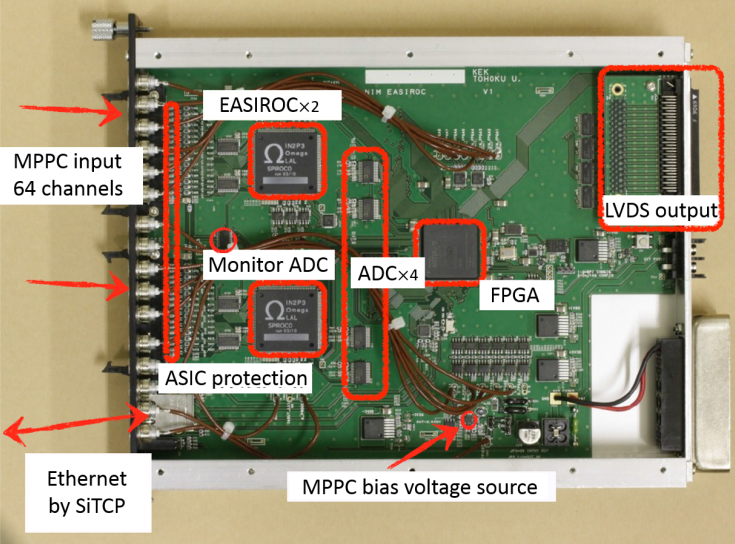
\includegraphics[width = 10.0cm, bb= 0 0 735 544]{2.png}
\end{center}
\caption{NIM-EASIROCボードの側面}
\label{fig:}
\end{figure}

\begin{figure}[H]
\begin{center}
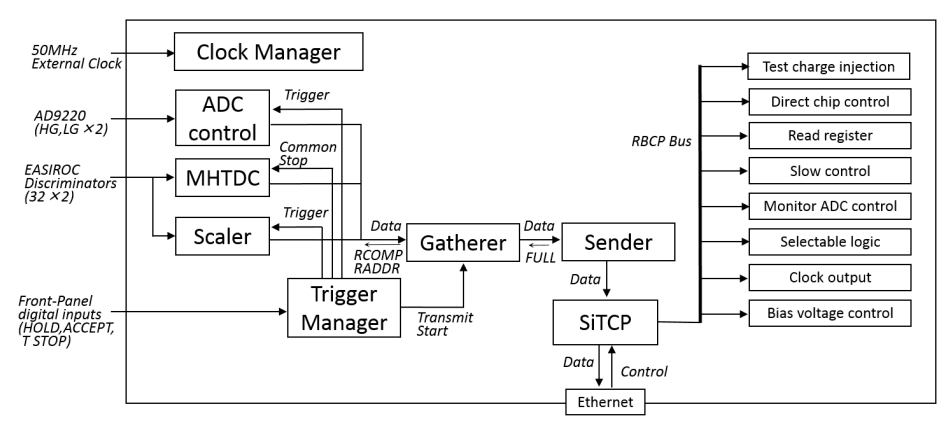
\includegraphics[width = 10.0cm, bb= 0 0 952 424]{3.png}
\end{center}
\caption{NIM-EASIROCボードの回路イメージ}
\label{fig:}
\end{figure}

\begin{figure}[H]
\begin{center}
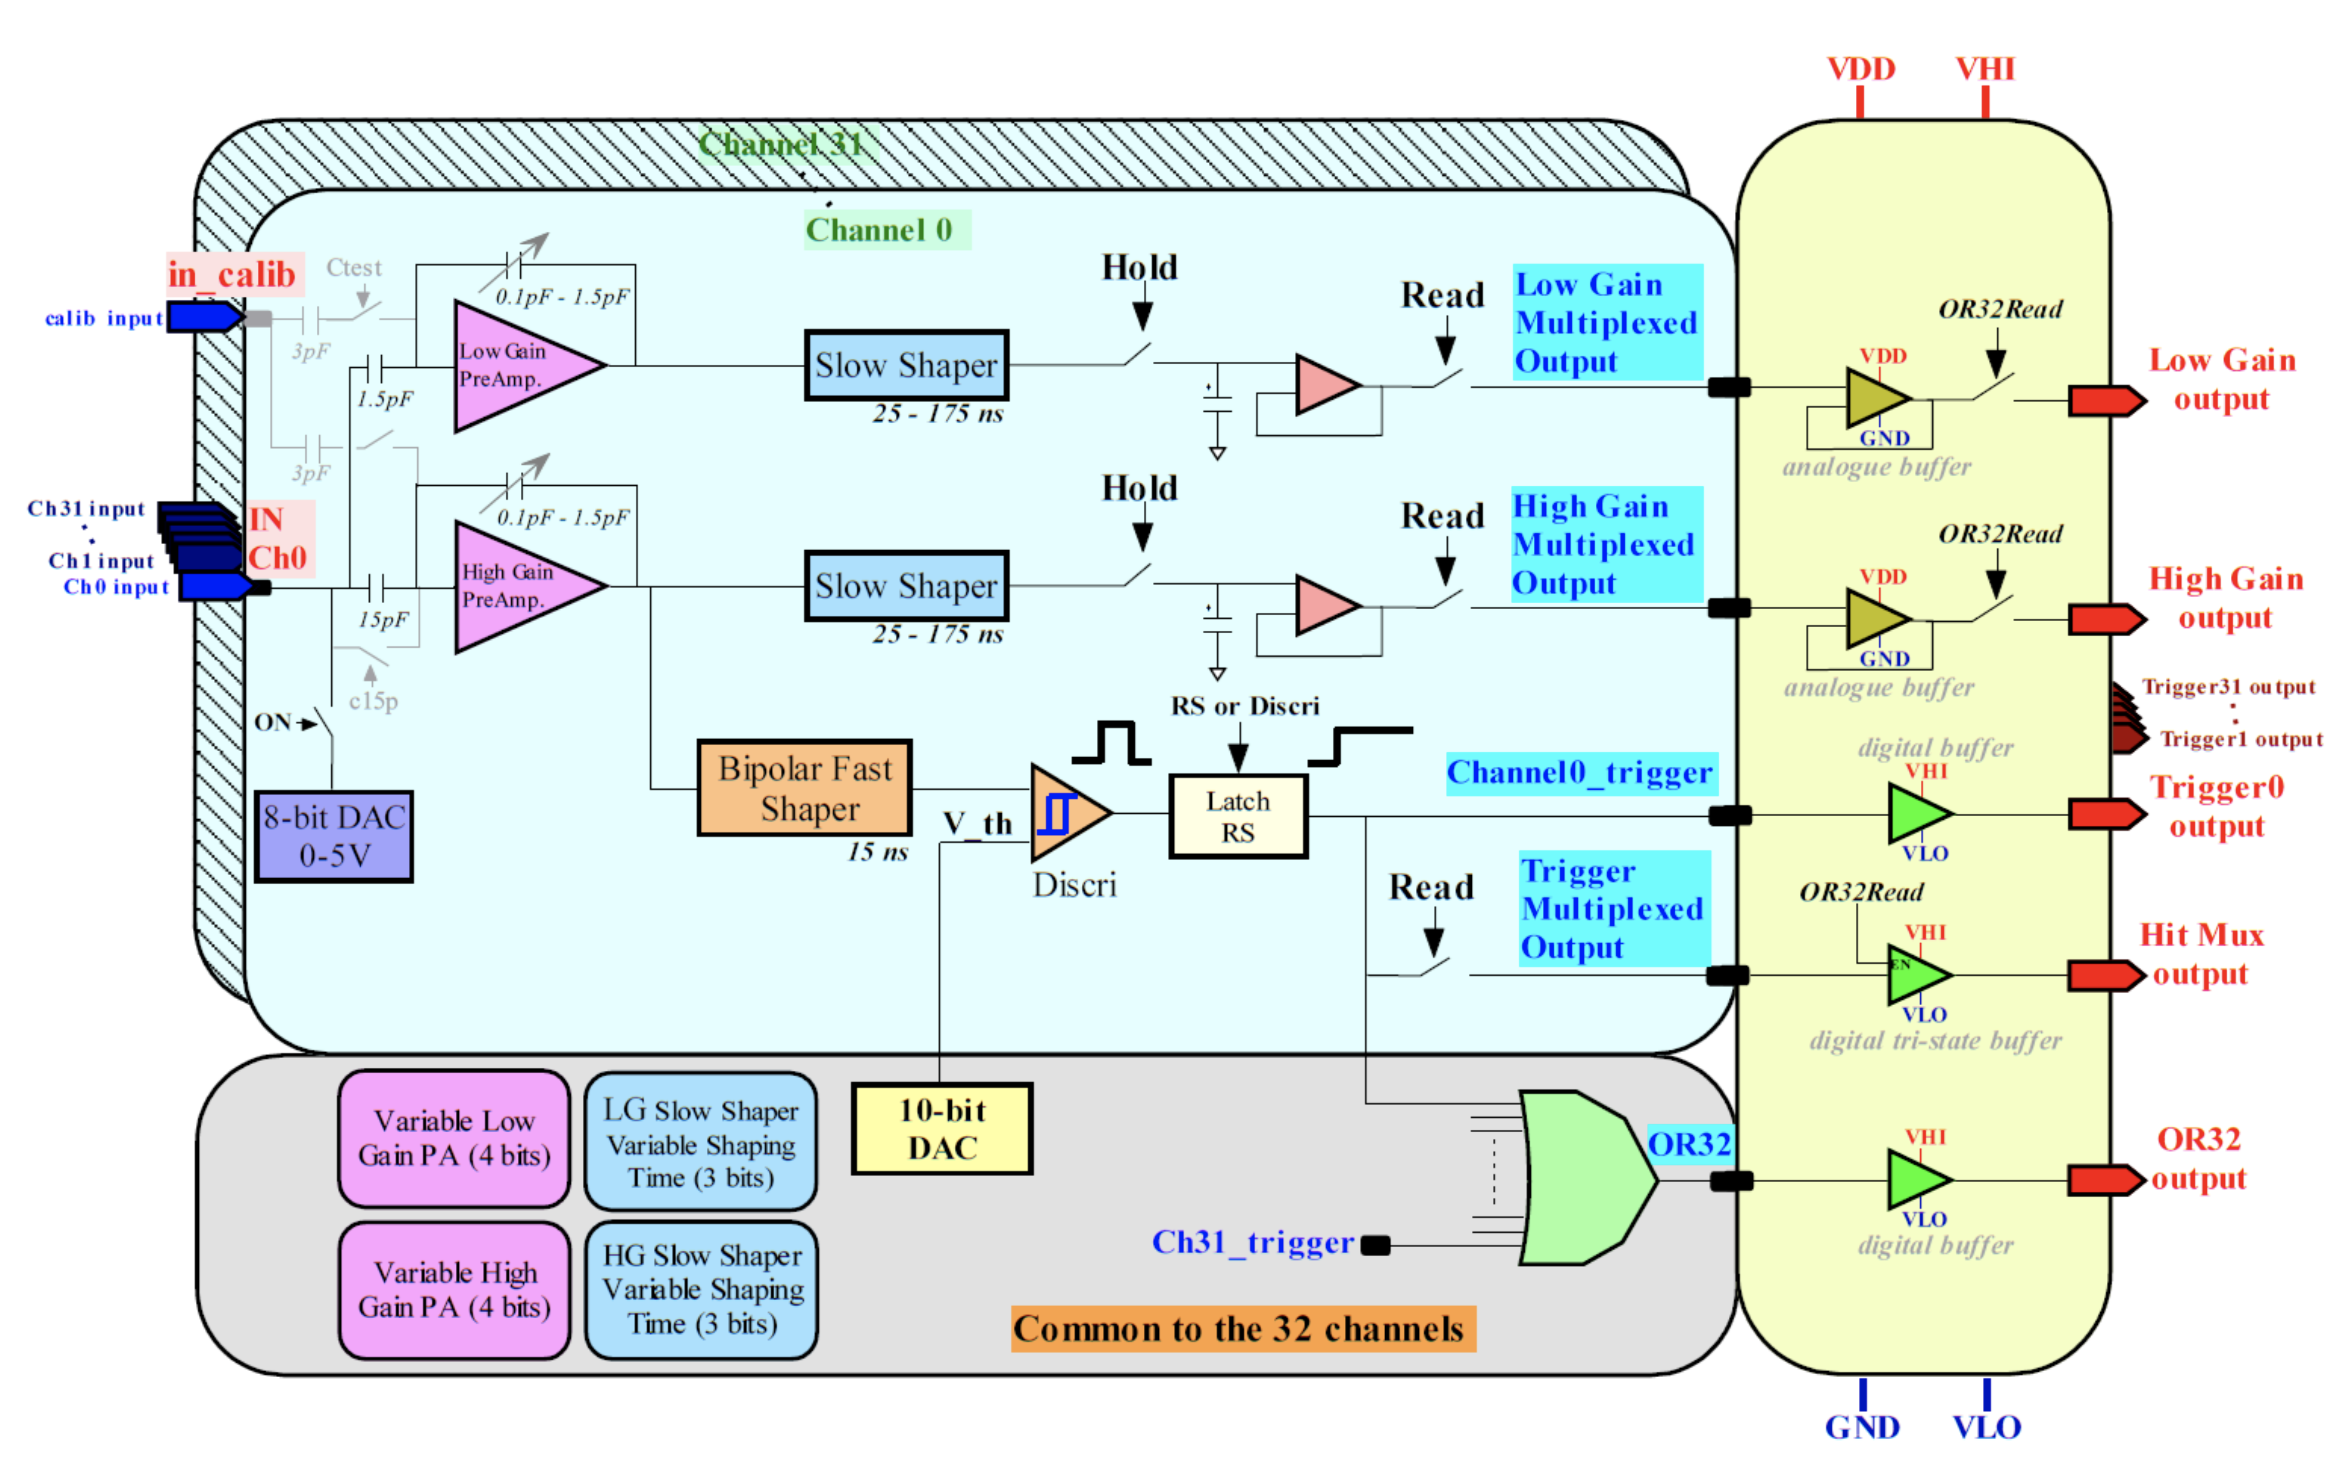
\includegraphics[width = 13.0cm, bb= 0 0 1167 735]{5.png}
\end{center}
\caption{EASIROC チップのブロックダイアグラム}
\label{fig:}
\end{figure}

アナログ信号の変換手順は以下のようになる。
\begin{enumerate}
\item Low 及び High 二つの異なるゲインを持つプリアンプにより電荷が積分・増幅される
\item プリアンプ出力は Fast shaper 及び Slow shaper に入力される
\item Fast shaper に入った信号は時定数 15 ns で整形され、Discriminator の Threshold を超えた場合にデジタル信号に変換される
\item Slow shaper に入った信号は時定数 25 - 175 ns で整形され、HOLD 信号を受け取った瞬間の電圧値が保持・記録される
\end{enumerate}



\section{How to Use EASIROC}
\subsection{Trigger signals}
Basically, only external trigger can be used. When you want to use self trigger, use output signals with appropriate delay. In that case, you should enter the signal with the order; "HOLD", "T STOP", "ACCEPT". 
You should insert more than about 2 us between HOLD and ACCEPT. It depends on ADC converting rate but 2.5 us is maybe enough.

\begin{figure}[H]
\begin{center}
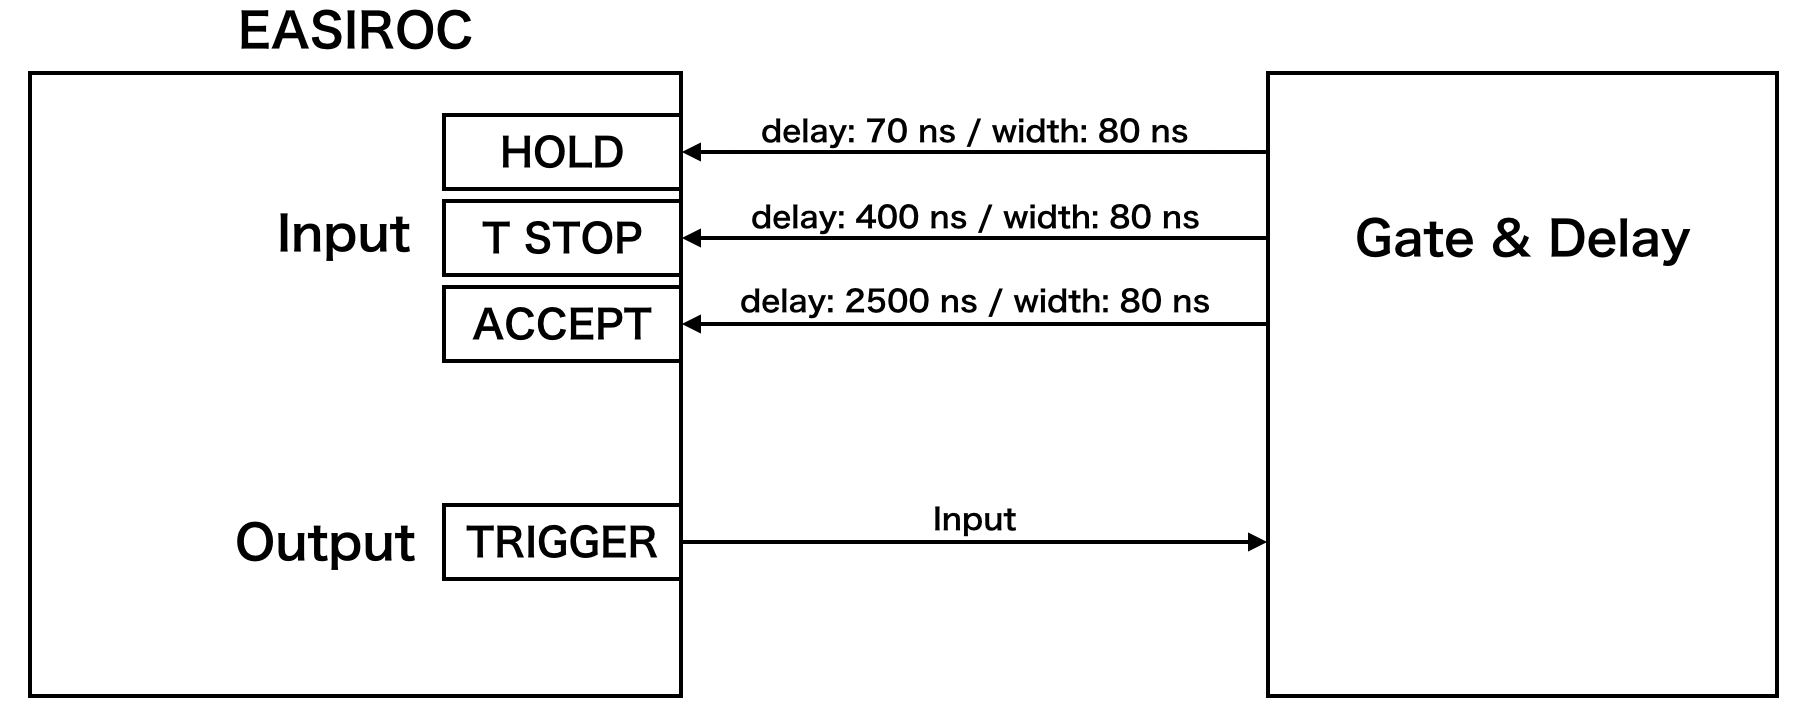
\includegraphics[width = 13.0cm, bb= 0 0 899 358]{1.png}
\end{center}
\caption{An example of self trigger circuit[1]}
\label{fig:}
\end{figure}

\begin{figure}[H]
\begin{center}
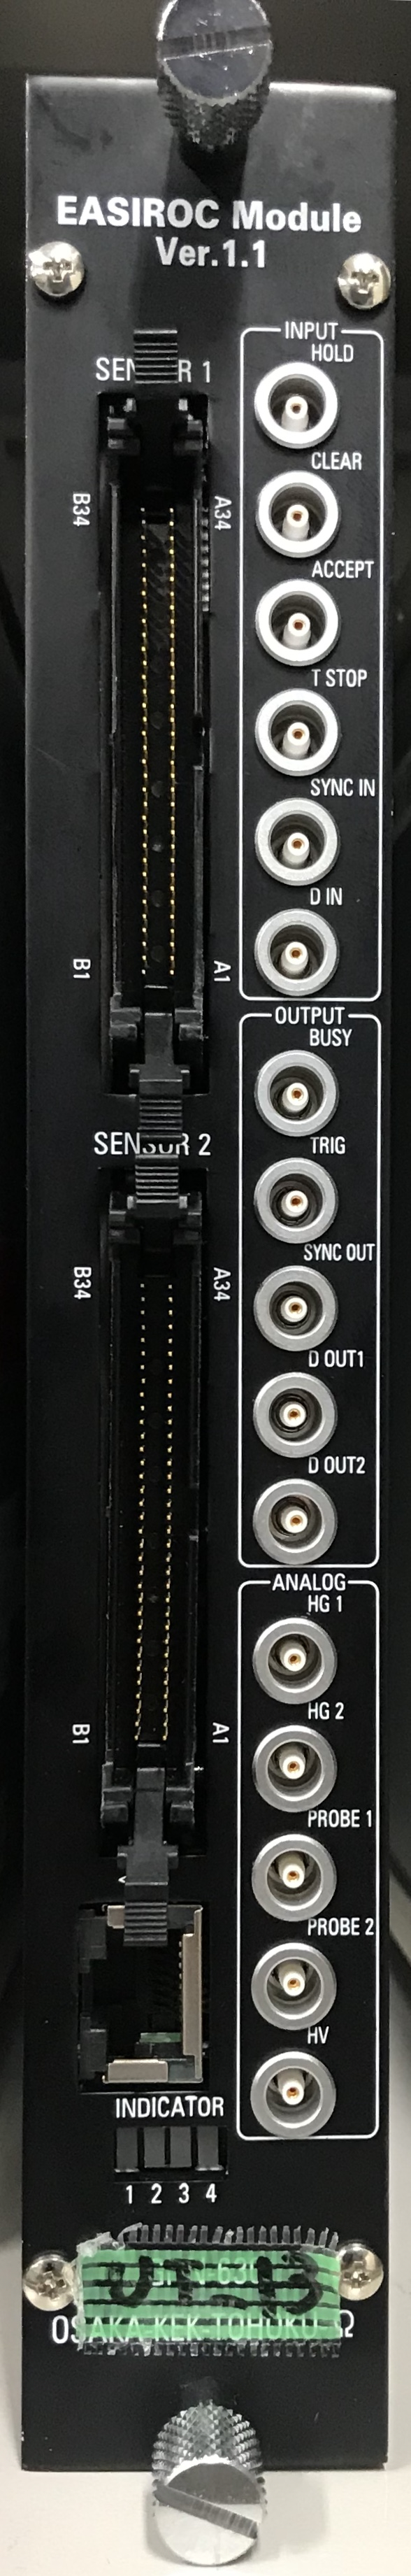
\includegraphics[width = 1.3cm, bb= 0 0 588 3683]{4.jpg}
\end{center}
\caption{The front panel of EASIROC board}
\label{fig:}
\end{figure}

\newpage
\subsection{Interactive mode}
EASIROC has an inner read line so you can handle EASIROC module interactively.

\subsubsection{Handle interactive mode}
Start interactive mode.
\begin{shadebox}
\begin{verbatim}
$ ./Controller.rb [IP Address (default: 192.168.10.16)]
\end{verbatim}
\end{shadebox}
 \\
Stop interactive mode.
\begin{shadebox}
\begin{verbatim}
> exit [quit]
\end{verbatim}
\end{shadebox}


\subsubsection{Set bias voltage}

Print the voltage and current value of HV.
\begin{shadebox}
\begin{verbatim}
> statusHV
\end{verbatim}
\end{shadebox}
 \\
Set the HV at the value of [bias voltage].
\begin{shadebox}
\begin{verbatim}
> setHV [bias voltage]
\end{verbatim}
\end{shadebox}
 \\
Increase HV with some steps. In each step, check the current and stop if it reaches to the limit.
\begin{shadebox}
\begin{verbatim}
> increaseHV [bias voltage]
\end{verbatim}
\end{shadebox}

\subsubsection{Data taking}
Reset the slow control values.
\begin{shadebox}
\begin{verbatim}
> slowcontrol
\end{verbatim}
\end{shadebox}
 \\
Start data aquisition.
\begin{shadebox}
\begin{verbatim}
> read [Event #] [Filename]
\end{verbatim}
\end{shadebox}
 \\
ON/OFF the ADC [TDC/Scaler].
\begin{shadebox}
\begin{verbatim}
> adc [on/off]
> tdc [on/off]
> scaler [on/off]
\end{verbatim}
\end{shadebox}
It makes data taking faster if you off the ADC [TDC/Scaler] when you don't need them.

\subsubsection{Other information}
\begin{itemize}
\item 対話時に入力されたコマンドは CommandDispatcher クラスによって処理される
\item 対話モードでhelp と入力してヘルプが見られる
\item 各コマンドは変数 COMMANDS に含まれているものが利用可能で、それぞれのコマンドはメソッドによって処理される
\item シェルのコマンドも一部使えるようになっている(ex. ls, mv, root)
\item それらは変数 DIRECT\_COMMANDS に含まれているものが利用可能
\item Controller ディレクトリ内で hist.cc を make してプログラムを生成していれば、read 終了後に自動でヒストグラムを生成する。出力先は Controller/data ディレクトリ内。
\end{itemize}

\newpage
\subsection{Slow Controll}
Slow Controll は yaml ディレクトリ下の YAML ファイル(拡張子:yml)によって指定される。\\
YAML は構造化されたデータを表現するフォーマットで、XML と似ているが YAML の方が人間にとって理解しやすい形式になっている。よく使いそうなものを以下に紹介する。

\subsubsection{RegisterValue.yml}

\begin{shadebox}
\begin{verbatim}
EASIROC1:  # Set for each chip
         Capacitor HG PA Fdbck: 100fF  # Define amplifying level. Capacitor values
         Capacitor LG PA Fdbck: 100fF  # are contained in RegisterValueAlias.yml
         Time Constant HG Shaper: 100ns  # Time constant of slow-shaper
         Time Constant LG Shaper: 50ns
         DAC code: 600  # Threshold of the discriminator after fast-shaper
 
EASIROC2:
         Capacitor HG PA Fdbck: same
         Capacitor LG PA Fdbck: same
         Time Constant HG Shaper: same
         Time Constant LG Shaper: same
         DAC code: same
 
High Gain Channel 1: 0   # Read out channel from HG1/HG2
High Gain Channel 2: -1  # 0 : read out || 1 : not read out
Probe Channel 1: -1      # Output from the probe of front panel
Probe Channel 2: -1
Probe 1: Out_fs
Probe 2: Out_fs  # Out_PA_HG, Out_PA_LG, Out_ssh_HG, Out_ssh_LG, Out_fs
SelectableLogic:
         Pattern: Or64        # OneCh_#, Or32u, Or32d, Or64, Or32And,...
         HitNum Threshold: 4  # Threshold for each OR logic. 0~64. Default: 0
         And Channels: -1     # Cannels used in And Logic. 0~63. Default: -1
TimeWindow: 4095ns
UsrClkOut: "OFF"  # Periodic signal from syn out of front panel # "ON", 1Hz,...
Trigger:          ## This "Trigger" values are not used for this version.
         Mode: 0  #0-7
         DelayTrigger: -1   #500MHz #default:-1, 0-253 #trig -> hold -> l1 -> l2
         DelayHold: -1      #25MHz
         DelayL1Trig: -1    #6MHz
         Width: raw
\end{verbatim}
\end{shadebox}

When increase the DAC of discriminator, threshold get lower.

\subsubsection{InputDAC.yml}
There written the 8-bit Input DAC values for 32 channels by chip. They can be changed between 256-511 (The top bit is always set to 1 (=enable)).\\
When increase the DAC value, bias voltage get lower. 

\begin{shadebox}
\begin{verbatim}
---
EASIROC1:
  Input 8-bit DAC:
  - 350
  - 350
  - 350
  - 350
  - 350
  - 350
  - 350
  - 350
\end{verbatim}
\end{shadebox}

\subsubsection{Calibration.yml}

\begin{shadebox}
\begin{verbatim}
HVControl:   # Coefficient for converting the HV into DAC
        - 413.9 #423.06 #483.183
        - 747.8 #767.17 #780.0
MonitorADC:  # Coefficient for converting Monitor ADC values
             # into voltage, current and temperature
        HV: 0.00208 #0.3235 #0.00208
        HVOffset: 0.0355 #4.1694
        Current: 0.0364 #0.034
        InputDac: 0.00006866 #4.5/2^16 #0.0000685
        Temperature: 4500.0
\end{verbatim}
\end{shadebox}

\newpage
\subsection{Other information}

\subsubsection{Probe output}


\begin{multicols}{2}
信号処理中の中間信号を取り出すための Probe 出力ラインがフロントパネルに用意されている。出力することができる中間信号を以下に示す。
\begin{itemize}
\item HighGain PreAmp 出力
\item LowGain PreAmp 出力
\item HighGain Slow shaper 出力
\item LowGain Slow shaper 出力
\item Fast shaper
\end{itemize}
前述の RegisterValue.yml から出力する情報を指定することができる。\\

PreAmp を選択した場合、波形全体ではなくピーク付近の一部のみ出力される。注意点としては、2 ch 以上を同時に ON にしない、データ取得中は Probe 1,2 を OFF にすること。


\begin{figure}[H]
\begin{center}
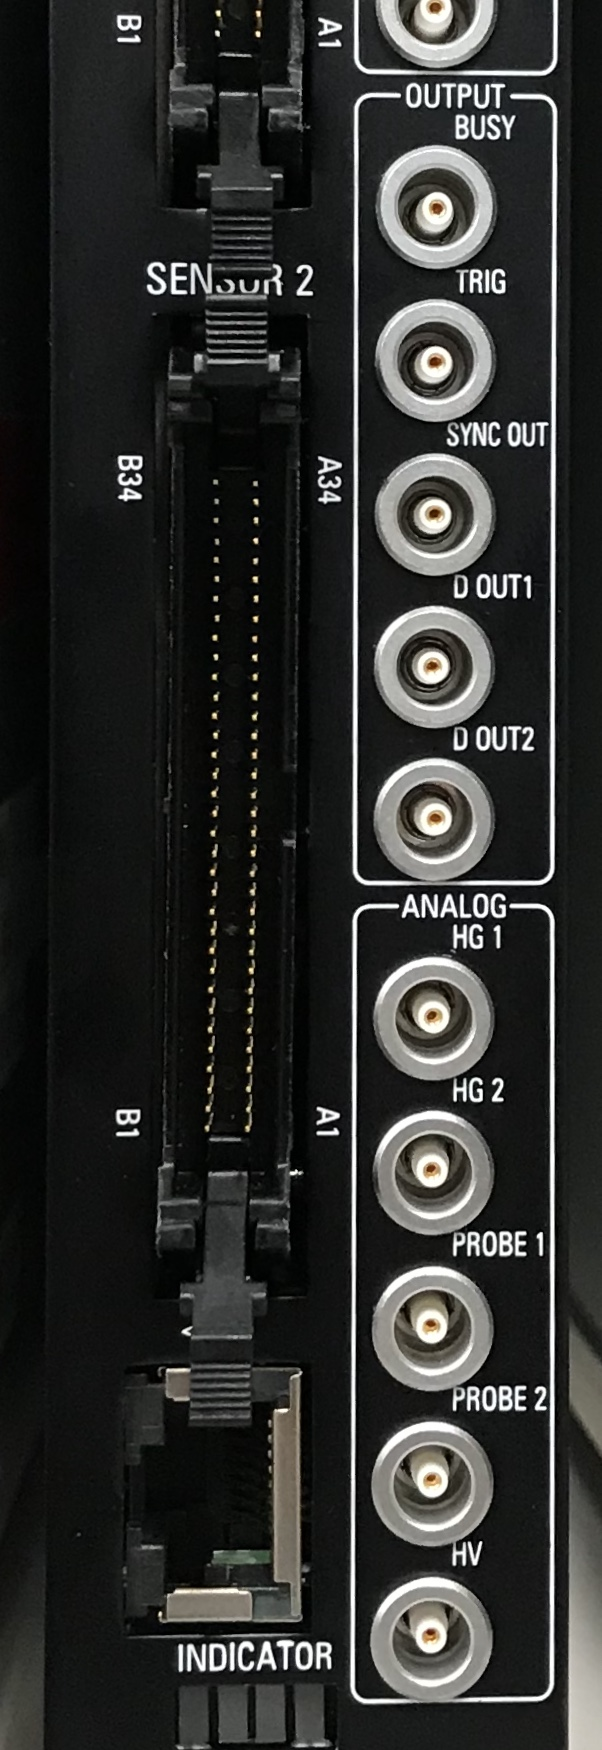
\includegraphics[width = 3cm, bb= 0 0 602 1750]{6.jpg}
\end{center}
\caption{フロントパネルの Probe 出力}
\label{fig:}
\end{figure}
\end{multicols}


\begin{shadebox}
\begin{verbatim}
High Gain Channel 1: 0   # HG で読み出すチャンネルの指定
High Gain Channel 2: -1  # 読み出すなら ch_#、読み出さないなら-1
Probe Channel 1: -1      # Probe からの出力チャンネル選択
Probe Channel 2: -1      # 2 ch 以上同時に使用しない
Probe 1: Out_PA_HG
Probe 2: Out_fs  # Out_PA_HG, Out_PA_LG, Out_ssh_HG, Out_ssh_LG, Out_fs
\end{verbatim}
\end{shadebox}
 \\
また、SYNC OUT からの周期信号も RegisterValue.yml より変更が可能である。

\begin{shadebox}
\begin{verbatim}
UsrClkOut: "OFF"  # "OFF", "ON", 1Hz, 10Hz, 100Hz, 1kHz, 10kHz, 100kHz, 3MHz, ...
\end{verbatim}
\end{shadebox}


\newpage
\subsubsection{Yokoyama-lab's EASIROCs}
2019年5月9日現在、5つの EASIROC ボードの存在が確認された。うち一つは京大高エネルギー研究室の備品と思われる。IP アドレスは DAC との接続の際に必要となる。
\begin{table}[H]
\begin{center}
\caption{横山研所有のEASIROC}
\begin{tabular}{ccc} \hline
管理No. & IP Adress & 備考 \\ \hline
1 & 192.168.10.11 &  \\ 
2 & 192.168.10.12 &  \\ 
3 & 192.168.10.13 &  \\ 
2号 & 192.168.10.18 & ch.32 の読み出し不調。バイアス HV にふらつきあり。 \\ 
京大高エネ備品 & 不明 & 後半 32ch の InputDAC が動かない。連絡先:075-753-3837。  \\ \hline
\end{tabular}
\end{center}
\end{table}


\subsection{その他}

\subsubsection{Probe 出力}


\begin{multicols}{2}
信号処理中の中間信号を取り出すための Probe 出力ラインがフロントパネルに用意されている。出力することができる中間信号を以下に示す。
\begin{itemize}
\item HighGain PreAmp 出力
\item LowGain PreAmp 出力
\item HighGain Slow shaper 出力
\item LowGain Slow shaper 出力
\item Fast shaper
\end{itemize}
前述の RegisterValue.yml から出力する情報を指定することができる。\\

PreAmp を選択した場合、波形全体ではなくピーク付近の一部のみ出力される。注意点としては、2 ch 以上を同時に ON にしない、データ取得中は Probe 1,2 を OFF にすること。


\begin{figure}[H]
\begin{center}
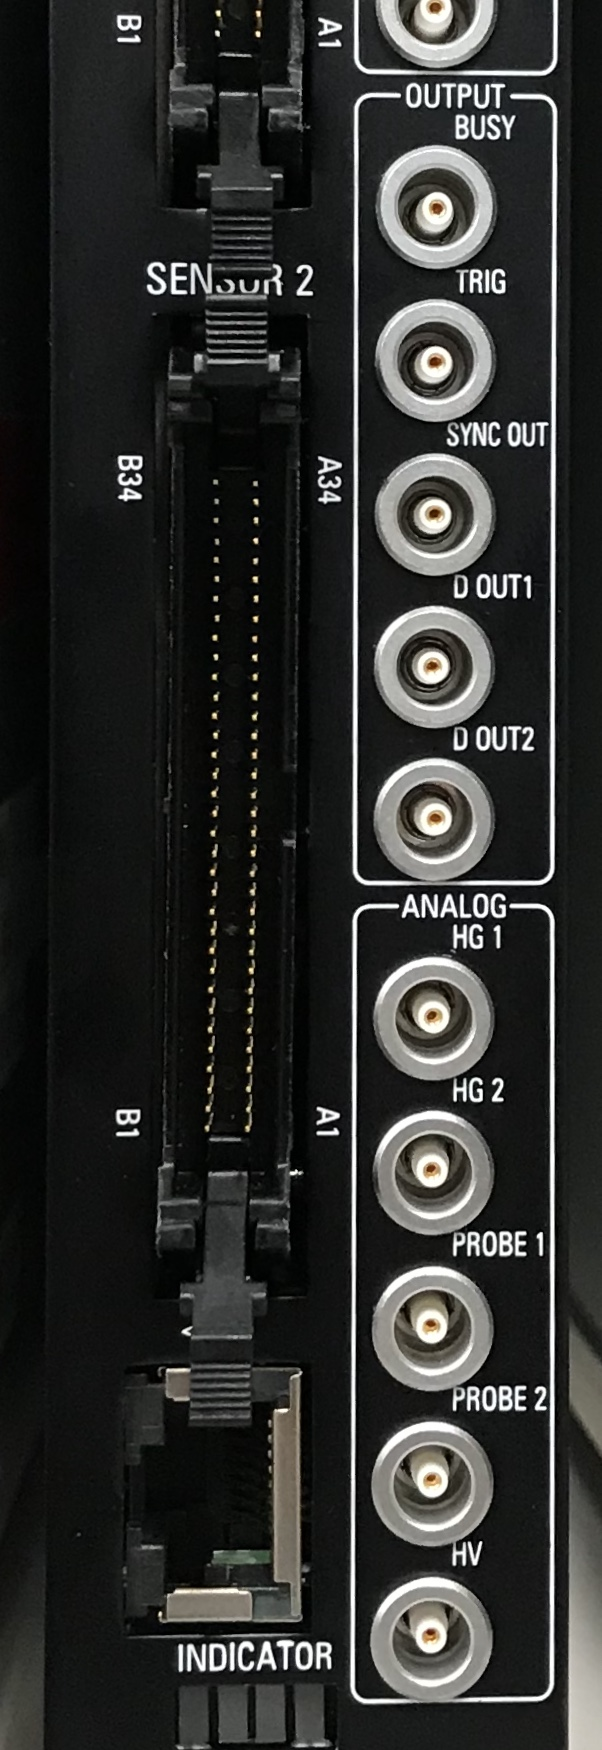
\includegraphics[width = 3cm, bb= 0 0 602 1750]{6.jpg}
\end{center}
\caption{フロントパネルの Probe 出力}
\label{fig:}
\end{figure}
\end{multicols}


\begin{shadebox}
\begin{verbatim}
High Gain Channel 1: 0   # HG で読み出すチャンネルの指定
High Gain Channel 2: -1  # 読み出すなら ch_#、読み出さないなら-1
Probe Channel 1: -1      # Probe からの出力チャンネル選択
Probe Channel 2: -1      # 2 ch 以上同時に使用しない
Probe 1: Out_PA_HG
Probe 2: Out_fs  # Out_PA_HG, Out_PA_LG, Out_ssh_HG, Out_ssh_LG, Out_fs
\end{verbatim}
\end{shadebox}
 \\
また、SYNC OUT からの周期信号も RegisterValue.yml より変更が可能である。

\begin{shadebox}
\begin{verbatim}
UsrClkOut: "OFF"  # "OFF", "ON", 1Hz, 10Hz, 100Hz, 1kHz, 10kHz, 100kHz, 3MHz, ...
\end{verbatim}
\end{shadebox}


\newpage
\subsubsection{横山研所有のEASIROC}
2019年5月9日現在、5つの EASIROC ボードの存在が確認された。うち一つは京大高エネルギー研究室の備品と思われる。IP アドレスは DAC との接続の際に必要となる。
\begin{table}[H]
\begin{center}
\caption{横山研所有のEASIROC}
\begin{tabular}{ccc} \hline
管理No. & IP Adress & 備考 \\ \hline
1 & 192.168.10.11 &  \\ 
2 & 192.168.10.12 &  \\ 
3 & 192.168.10.13 &  \\ 
2号 & 192.168.10.18 & ch.32 の読み出し不調。バイアス HV にふらつきあり。 \\ 
京大高エネ備品 & 不明 & 後半 32ch の InputDAC が動かない。連絡先:075-753-3837。  \\ \hline
\end{tabular}
\end{center}
\end{table}


\newpage
\section{参考文献}
1,2,3 は EASIROC 開発時の資料、4,5 はアップグレード後の資料である。
\begin{enumerate}
\item OpenIt のサイト\\
\url{http://openit.kek.jp/project/MPPC-Readout-Module/public/MPPC-Readout-Module}
\item 石島さんの修論\\
\url{http://osksn2.hep.sci.osaka-u.ac.jp/theses/master/2013/ishijima_mthesis.pdf}
\item 塩崎さんの修論\\
\url{http://lambda.phys.tohoku.ac.jp/~db/human_resource/thesis/2009_B_2_M_1.pdf}
\item 竹馬さんのマニュアル\\
\url{http://hep.phys.s.u-tokyo.ac.jp/~nchikuma/easiroc_manual.html} 
\item 竹馬さんの修論\\
\url{http://hep.phys.s.u-tokyo.ac.jp/wordpress/wp-content/uploads/2016/06/mth2016_chikuma.pdf}
\end{enumerate}

\end{document}





\end{document}



